\documentclass[11pt,a4paper]{article}
\usepackage[a4paper,margin=0.72in]{geometry}
\usepackage{graphicx}
\usepackage{booktabs}
\usepackage{longtable}
\usepackage{tabularx}
\usepackage{array}
\usepackage{enumitem}
\usepackage{hyperref}
\usepackage{listings}
\usepackage{float}
\hypersetup{colorlinks=true,urlcolor=black,linkcolor=black,citecolor=black}
\setlist{nosep}
\renewcommand{\arraystretch}{1.15}
\newcolumntype{Y}{>{\raggedright\arraybackslash}X}
\title{\textbf{Design Pattern Analysis in a Flask-Based Event Management Application}}
\author{Team A15\[2mm]
Harshitha D --- AM.SC.U4CSE23222\\
T Heshaja --- AM.SC.U4CSE23265}
\date{2026-10-06}
\begin{document}
\maketitle
\tableofcontents
\newpage

\section{Application and Architecture}
\subsection{Application}
The selected application is an Event Management System implemented as a Python/Flask web application. It supports organizer and attendee workflows including authentication, event creation and management, event discovery, ticket registration, and ticket management. The supplied repository also contains a PHP subtree; that subtree was excluded from the case-study analysis because the assigned case is specifically the Flask-based application.

\subsection{Original Source and Environment}
\begin{itemize}
\item Source repository: \url{https://github.com/ARUNAGIRINATHAN-K/Event-Management-system}
\item Access/inspection date: 2026-10-06.
\item Baseline source: repository ZIP snapshot supplied for this case study. The ZIP did not preserve a Git commit hash, so no commit identifier is invented.
\item Python requirement: $\geq$3.11.
\item Locked dependency versions: Flask 3.1.0, Flask-Login 0.6.3, Flask-SQLAlchemy 3.1.1, Flask-WTF 1.2.2, SQLAlchemy 2.0.40.
\item Persistence: SQLAlchemy ORM; the application uses a configured database URL with a SQLite fallback in the source.
\end{itemize}

\subsection{Scope and Architecture}
The inspected baseline scope includes \texttt{app.py}, \texttt{models.py}, \texttt{forms.py}, \texttt{routes.py}, \texttt{utils.py}, templates, static assets, and configuration/dependency files. The PHP subtree was excluded. The baseline request path for event creation is a controller route that validates an \texttt{EventForm}, constructs an \texttt{Event}, writes through \texttt{db.session}, and renders or redirects through the template layer.

\begin{figure}[H]
\centering
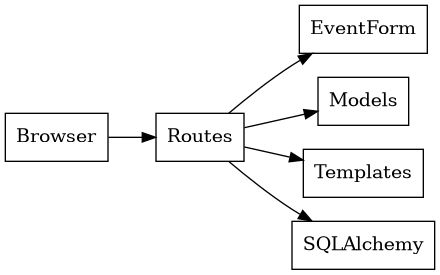
\includegraphics[width=0.92\linewidth]{code/architecture/baseline.png}
\caption{Baseline Flask application architecture.}
\end{figure}

After refactoring, the route layer delegates persistence to repositories, filtering to strategies, and registration side effects to an observer-enabled registration service.
\begin{figure}[H]
\centering
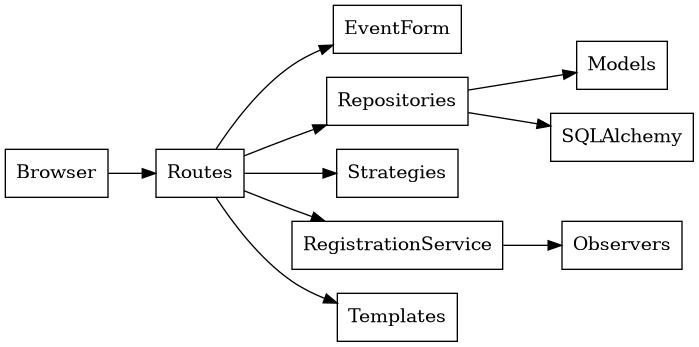
\includegraphics[width=0.92\linewidth]{code/architecture/evolved.png}
\caption{Evolved architecture after CH01--CH03.}
\end{figure}

\subsection{Run and Verification}
The supplied project declares its dependencies in \texttt{pyproject.toml} and locks versions in \texttt{uv.lock}. The structural pattern test command used for the refactored source was:
\begin{verbatim}
python3 tests/test_design_patterns.py
\end{verbatim}
Actual result: 4 tests passed. The full Flask application was not claimed as runtime-tested in the verification container because the Flask runtime dependency was unavailable there; this limitation is preserved rather than replaced with an estimated result.

\section{Part 1 Pattern Discovery}
\subsection{Method}
Candidates were identified from source structure and behavior, then checked against actual collaborations: participants, calls/delegation, responsibilities, and evidence in source. A class name, decorator annotation, or LLM assertion alone was not treated as sufficient evidence. Candidate patterns that lacked the required collaboration were rejected.

\subsection{Baseline Totals}
\begin{itemize}
\item Confirmed pattern types: \textbf{4}.
\item Confirmed pattern instances: \textbf{4} independent collaborations.
\item Concrete participant classes: \textbf{3} distinct classes across the baseline records (\texttt{EventForm}, \texttt{Event}, \texttt{Ticket}); functions, decorators, templates, and objects are not counted as classes.
\item Unique participant symbols: \textbf{12} after deduplication across the four baseline records.
\item Rejected candidates: Singleton, Strategy, Observer, Facade.
\item Uncertain candidates: none retained as confirmed baseline patterns.
\end{itemize}

\subsection{Pattern Inventory}
\begin{longtable}{p{0.22\linewidth}p{0.34\linewidth}p{0.16\linewidth}p{0.20\linewidth}}
\toprule
Pattern & Instance & Type & Instances\\
\midrule
MVC & Event Creation MVC Flow & Architectural & 1\\
Decorator & Authenticated Event Route Registration & Framework idiom & 1\\
Active Record-like ORM & Event and Ticket Persistence Model & Architectural/Data Access & 1\\
Form Object & Event Creation Validation & Framework/Application idiom & 1\\
\bottomrule
\end{longtable}

\subsection{Confirmed Pattern Records}
\subsubsection{Event Creation MVC Flow}
\textbf{Pattern/category:} MVC / architectural.\\
\textbf{Origin:} Application architecture.\\
\textbf{Participants:} controller = \texttt{routes.register\_routes.create\_event}; form = \texttt{forms.EventForm}; model = \texttt{models.Event}; view = \texttt{templates/organizer/create\_event.html}; persistence = \texttt{db.session}.\\
\textbf{Evidence:} the controller creates and validates the form, constructs an Event, commits it through the SQLAlchemy session, then redirects or renders the template. Baseline source locations are \texttt{routes.py:118--149}, \texttt{forms.py:43--61}, and \texttt{models.py:50--86}.\\
\textbf{Verification:} confirmed from source behavior; no separate MVC framework class hierarchy was invented.

\subsubsection{Authenticated Event Route Registration}
\textbf{Pattern/category:} Decorator / framework idiom.\\
\textbf{Participants:} Flask route decorator, Flask-Login \texttt{login\_required}, and decorated \texttt{logout} function.\\
\textbf{Evidence:} \texttt{routes.py:95--100} shows \texttt{@app.route('/logout')} and \texttt{@login\_required} wrapping the route function. The authentication behavior is added around the function without changing its body. This is reported as a framework/Python decorator idiom rather than a complete GoF Decorator subsystem.\\
\textbf{Verification:} confirmed.

\subsubsection{Event and Ticket Persistence Model}
\textbf{Pattern/category:} Active Record-like ORM / architectural-data access.\\
\textbf{Participants:} \texttt{models.Event}, \texttt{models.Ticket}, SQLAlchemy \texttt{db}, and route-level query/session operations.\\
\textbf{Evidence:} Event and Ticket combine persistent fields with domain behavior while the baseline routes directly query, create, and commit these objects. Key locations are \texttt{models.py:50--114}, \texttt{app.py:17--33}, \texttt{routes.py:130--144}, and \texttt{routes.py:328--371}.\\
\textbf{Verification:} confirmed as an Active Record-like ORM collaboration; it is not claimed to be a pure textbook Active Record implementation.

\subsubsection{Event Creation Validation}
\textbf{Pattern/category:} Form Object / framework-application idiom.\\
\textbf{Participants:} \texttt{forms.EventForm}, its date validators, the event creation controller, and the event creation template.\\
\textbf{Evidence:} \texttt{EventForm} encapsulates event fields and cross-field validation; the controller calls \texttt{validate\_on\_submit()} before creating the model. Locations include \texttt{forms.py:43--61} and \texttt{routes.py:118--149}.\\
\textbf{Verification:} confirmed.

\subsection{Rejected Candidates}
\begin{itemize}
\item \textbf{Singleton:} module-level Flask/SQLAlchemy objects are not evidence of an explicit Singleton implementation with controlled construction/access.
\item \textbf{Strategy:} baseline event filtering is implemented directly with conditional query modifications in \texttt{routes.py:275--291}; there are no interchangeable strategy objects.
\item \textbf{Observer:} baseline registration creates and commits tickets directly and has no subject/observer subscription collaboration.
\item \textbf{Facade:} utility functions did not provide sufficiently clear evidence of one unified subsystem facade, so the candidate was not counted.
\end{itemize}

\section{Part 2 Evolution and Refactoring}
Each change was implemented as a real code modification and represented as a new collaboration only when the source showed the corresponding participants and behavior. The final evolution CSV preserves the baseline rows and appends the post-change snapshots.

\subsection{CH01 --- Repository Pattern}
\textbf{Requirement:} remove direct persistence/query responsibilities from Flask route handlers.\\
\textbf{Before:} routes directly used \texttt{Event.query}, \texttt{Ticket.query}, \texttt{db.session.add}, and \texttt{db.session.commit}.\\
\textbf{After:} \texttt{EventRepository}, \texttt{TicketRepository}, and \texttt{UserRepository} encapsulate query and persistence operations. Routes obtain domain objects through repository methods.\\
\textbf{Pattern effect:} Repository --- newly introduced. The existing MVC and ORM collaborations are modified because persistence is now mediated by repositories.\\
\textbf{Verification:} structural test suite 4/4 passed; modified Python files compile.\\
\textbf{Refactoring rationale:} the route module mixed HTTP/controller responsibilities with persistence mechanics, creating a separation-of-concerns problem.

\subsection{CH02 --- Strategy Pattern}
\textbf{Requirement:} make event filtering criteria interchangeable.\\
\textbf{Before:} the attendee event route contained separate conditional query filters for text, category, start date and end date.\\
\textbf{After:} \texttt{EventFilterStrategy} defines the strategy contract; text, category and date-range strategies implement it. The route selects active strategies and \texttt{EventRepository.search\_upcoming()} applies them sequentially.\\
\textbf{Pattern effect:} Strategy --- newly introduced.\\
\textbf{Verification:} structural tests and Python compilation passed.\\
\textbf{Refactoring rationale:} the route's conditional filtering logic was a direct collection of policy branches; strategies isolate each criterion and permit additional criteria without rewriting the repository's application loop.

\subsection{CH03 --- Observer Pattern}
\textbf{Requirement:} decouple registration side effects from the registration route.\\
\textbf{Before:} the route created and committed tickets itself.\\
\textbf{After:} \texttt{EventRegistrationService} acts as the subject. It creates tickets through \texttt{TicketRepository}, then notifies attached \texttt{RegistrationNotificationObserver} and \texttt{RegistrationStatisticsObserver} instances.\\
\textbf{Pattern effect:} Observer --- newly introduced.\\
\textbf{Verification:} structural tests and Python compilation passed.\\
\textbf{Refactoring rationale:} ticket creation and post-registration reactions are separated so new reactions can be attached without adding more side-effect code to the route.

\subsection{Updated Pattern Counts}
\begin{longtable}{p{0.25\linewidth}p{0.18\linewidth}p{0.16\linewidth}p{0.18\linewidth}}
\toprule
Snapshot & Pattern types & Pattern instances & Newly introduced\\
\midrule
Original & 4 & 4 & --\\
After CH01 & 5 & 5 & Repository\\
After CH02 & 6 & 6 & Strategy\\
After CH03 & 7 & 7 & Observer\\
\bottomrule
\end{longtable}

\subsection{Before/After Metrics}
Using the same source-LOC rule (nonblank, non-comment production lines), \texttt{routes.py} decreased from 340 LOC to 336 LOC. The new repository, strategy, observer and service modules add 193 nonblank, non-comment lines. This demonstrates responsibility movement rather than a claim that fewer total lines automatically means better design. Complexity/timing for the small cross-language snippets is recorded separately in \texttt{data/cross\_language.csv}.

\section{Part 3 Cross-Language Comparison}
\subsection{Selected Instances and Common Specification}
The three newly introduced patterns were selected because they represent the actual Part 2 refactorings. Each was reduced to a small deterministic problem and implemented in Java, Python, JavaScript and C++. The same conceptual inputs and expected outputs were used within each pattern family.

\begin{itemize}
\item \textbf{Repository:} store events and retrieve an event by identifier.
\item \textbf{Strategy:} filter a common event set using interchangeable name/category criteria.
\item \textbf{Observer:} register an attendee and produce both notification and statistics reactions.
\end{itemize}

Compilation/interpreter versions, commands, source LOC, maximum function cyclomatic complexity, test result, median process time and language notes are stored in \texttt{data/cross\_language.csv}. The timing protocol was compile first, one warmup, five measured process runs, then median. Timing includes process startup and test execution.

\subsection{Measured Results}
\begin{longtable}{p{0.16\linewidth}p{0.14\linewidth}r r r}
\toprule
Pattern & Language & LOC & Max CC & Median ms\\
\midrule
Repository & Java & 3 & 1 & 24.629\\
Repository & Python & 11 & 1 & 594.444\\
Repository & JavaScript & 8 & 1 & 21.222\\
Repository & C++ & 6 & 1 & 1.105\\
Strategy & Java & 6 & 2 & 26.806\\
Strategy & Python & 13 & 1 & 567.115\\
Strategy & JavaScript & 5 & 1 & 21.456\\
Strategy & C++ & 11 & 2 & 1.117\\
Observer & Java & 6 & 1 & 56.745\\
Observer & Python & 15 & 1 & 571.284\\
Observer & JavaScript & 4 & 1 & 22.141\\
Observer & C++ & 9 & 1 & 1.356\\
\bottomrule
\end{longtable}
All 12 implementations passed their tests. These values are process-level measurements on the same verification machine, not claims about the intrinsic performance of the languages or of the original Flask application.

\subsection{Static and Dynamic Comparison}
Java uses explicit interfaces/classes for the Strategy and Observer collaborations. Python uses lightweight classes and duck-typed collaboration, resulting in compact implementations. JavaScript uses object/class composition with less boilerplate. C++ uses explicit classes and compilation with C++17. The maximum function complexity remained low (1--2) because the representative problems were intentionally small. Runtime differences are dominated by process startup, interpreter/JVM initialization and the small workload, so they should not be interpreted as production performance rankings.

\section{LLM Records and Human Verification}
The project records three major AI-assisted analysis interactions in \texttt{data/llm.csv}, with prompt, output and verification files under the corresponding Part1/Part2/Part3 folders. The model displayed for these records was ChatGPT GPT-5.6 Luna on 2026-10-06.

\begin{longtable}{p{0.12\linewidth}p{0.22\linewidth}p{0.29\linewidth}p{0.29\linewidth}}
\toprule
Part & Analysis & Evaluation & Verification\\
\midrule
Part 1 & Baseline pattern inventory & Correct after source-based checking; unsupported candidates rejected & Source locations and collaboration behavior in baseline Flask code\\
Part 2 & Refactoring/evolution & Correct for implemented changes; runtime limitation explicitly retained & 4/4 structural tests and Python compilation\\
Part 3 & Cross-language analysis & Correct & 12/12 implementations passed; five-run median measurements\\
\bottomrule
\end{longtable}

The evidence files explicitly distinguish reconstructed/conversation-derived prompt context from verbatim historical files where applicable. No invented LLM experiment is presented as an actual run.

\section{Findings, Contributions and References}
\subsection{Findings}
\begin{enumerate}
\item The baseline Flask application already contains several recognizable architectural/framework idioms, but not every common GoF pattern is present. In particular, Strategy and Observer were not counted until concrete collaborations were introduced.
\item CH01 separates HTTP/controller concerns from persistence mechanics without removing the underlying SQLAlchemy model layer.
\item CH02 converts hard-coded filtering branches into independently selectable strategies.
\item CH03 separates registration side effects from the route and provides explicit extension points for new reactions.
\item Cross-language structure varies substantially in boilerplate and runtime behavior, while the representative pattern responsibilities remain comparable.
\item Source LOC alone is insufficient to establish a refactoring as better; the report therefore combines responsibility placement, pattern collaboration and test evidence with LOC measurements.
\end{enumerate}

\subsection{Limitations}
The baseline Git commit hash was not preserved in the supplied ZIP. Full Flask runtime execution was not available in the verification container, so only the actual structural/compilation result is reported. Cross-language timing is process-level and based on small deterministic snippets; it is not a benchmark of production systems. Individual team-member task allocation was not included in the supplied case-study materials and is therefore not invented.

\subsection{Team Contributions}
The four listed team members jointly constitute Team A15. The supplied materials identify membership but do not provide individual task allocation; consequently, the submission records team-level work rather than assigning unsupported individual roles.

\subsection{References}
\begin{enumerate}
\item 23CSE455 Design Pattern Case Study Instructions, supplied course PDF, accessed 2026-10-06.
\item 23CSE455 Design Patterns Case Study Report Template, supplied course PDF, accessed 2026-10-06.
\item Event Management System repository: \url{https://github.com/ARUNAGIRINATHAN-K/Event-Management-system}.
\item E. Gamma, R. Helm, R. Johnson and J. Vlissides, \emph{Design Patterns: Elements of Reusable Object-Oriented Software}, Addison-Wesley, 2000.
\item Flask documentation: \url{https://flask.palletsprojects.com/}.
\item SQLAlchemy documentation: \url{https://docs.sqlalchemy.org/}.
\end{enumerate}

\section{Team Folder and Dataset Map}
The final submission folder is \texttt{A15/}. It contains one report, one dataset directory, and supporting Part1/Part2/Part3 evidence. The five required CSV files occur only in \texttt{data/}.
\begin{verbatim}
A15/
  README.md
  A15_Report.pdf
  A15_Report.tex
  data/
    patterns.csv
    pattern_counts.csv
    patterns_evolution.csv
    cross_language.csv
    llm.csv
  code/
    original/
    architecture/
  Part1/
    code/
    evidence/
    llm/
  Part2/
    code/evolved/
    changes/Change1..Change3/
    evidence/
    llm/
  Part3/
    Repository/
    Strategy/
    Observer/
    test-cases/
    evidence/
    llm/
\end{verbatim}

\end{document}
